\section{Design \& Implementation} \label{design}
\subsection{Modulating Acceleration and Deceleration}
Swink discussed different ways to modulate the player avatar's movement in the chapter \textit{Response Metrics} \cite{swink}. Inspired by ADSR envelopes (Attack-Decay-Sustain-Release), Swink proposed the idea of using velocity modulation to change the game feel. Even if the input signal from the game controller is discrete and binary (button is either pressed down or released), the software can modulate it into a continuous signal. By altering the attack and release phase (or, acceleration and deceleration), it is possible to create different game feel, as illustrated in Figures \ref{fig:adsr_stiff} and \ref{fig:adsr_loose}.

%, e.g., the sound of a pipe organ or a guitar string. This is achieved by modulating the amplitude over time.

%Inspired by Swink's discussion about \textit{Response Metrics} \cite{swink}, a 2D platforming game was developed. The game changes two types of parameters between each round: how fast the ball accelerates and how fast it decelerates when moving horizontally. Swink calls these the \textit{attack} and \textit{release} phases, or, the acceleration and deceleration of avatar movement. Hence, the velocity of the player's avatar is modulated over time, creating different types of game feel. Figures \ref{fig:adsr_stiff} and \ref{fig:adsr_loose} show two examples of the modulations proposed by Swink.


%According to Swink, when the acceleration or deceleration is very long (e.g., the avatar takes more than 100 milliseconds to be perceived to be moving), the impression of instantaneous response erodes. Even if there are small changes in the velocity, if these cannot be perceived by the player, the game might feel unresponsive \cite{swink}. This is illustrated by Figure \ref{fig:adsr}.

\begin{figure}[htbp]
\centering
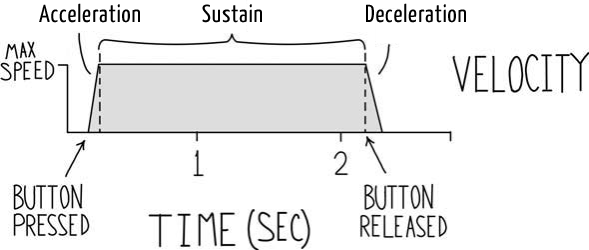
\includegraphics[width=0.30\textwidth]{Pics/adsr_stiff}
\caption{Short acceleration/deceleration gives a responsive, but stiff, feel. Figure inspired by Swink \cite{swink}.}
\label{fig:adsr_stiff}
\end{figure}

\begin{figure}[htbp]
\centering
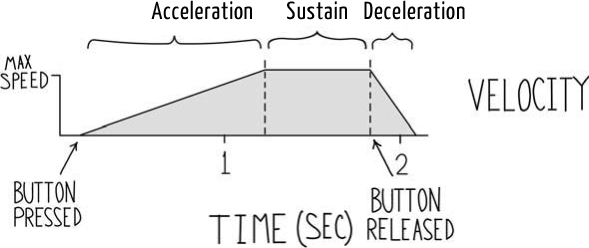
\includegraphics[width=0.30\textwidth]{Pics/adsr_loose}
\caption{Long acceleration gives a loose, but fluid, feel. Figure inspired by Swink \cite{swink}.}
\label{fig:adsr_loose}
\end{figure}

Taking inspiration from Swink, a 2D side-scrolling platformer game was developed in Unity. Using the keyboard, players control a soccer ball from left to right to collect stars (see Figure \ref{fig:game}). Two parameters change between each round: how fast the ball accelerates and how fast it decelerates (when moving horizontally). Hence, the velocity of the player's avatar is modulated over time. This means that when the player presses the movement button, the ball takes a certain amount of time before it reaches its maximum velocity. The same is applied when the player releases the button: the ball gradually slows down, until it stops.

%To keep the experiment as simple as possible, only linear curves were considered for this project. Also, the decay phase was deemed unnecessary, since it wouldn't make sense for an avatar to accelerate, then decay a little, and then sustain the maximum velocity.

%Depending on how big a delay there is from the player triggering an event to getting feedback, the game will gradually feel less responsive.

Two intervals were chosen, inspired by Swink's model of player perception and feedback. The first interval, \textit{fast}, is between 1 millisecond and 240 milliseconds. The second interval, \textit{slow}, is from 241 milliseconds to 1500 milliseconds. For each round in the game, the player is assigned randomly-chosen values within these two intervals. 
%The reason for choosing random values instead of fixed values is that it isn't perfectly clear at which exact point a game goes from feeling responsive to unresponsive. Instead of choosing arbitrary fixed numbers, the system randomly assigns numbers within the two intervals. 
The acceleration/deceleration is thus scaled depending on the time values, using Equation \ref{eq:erl}.
\begin{equation} \label{eq:erl} %% source: http://www.calculatorsoup.com/calculators/physics/velocity_a_t.php
a = (v - v_0)/{\Delta}t
\end{equation} 
where $a$ is the acceleration/deceleration, $v$ is the target velocity, $v_0$ is the initial velocity and ${\Delta}t$ is the time after which the target velocity is reached.

%\begin{table} \centering
%\label{tab:time}
%\caption{Time intervals for the acceleration/deceleration.}
%\begin{tabular}{cc}
%\toprule
%\textbf{Fast} & \textbf{Slow} \\
%\midrule
%1 ms - 240 ms & 241 ms - 1500 ms\\
%\bottomrule
%\end{tabular}
%\end{table}

The game features other parameters, such as gravity, jump velocity and the aforementioned ``ghost jump", but only the horizontal ground acceleration and deceleration changed between rounds. Graphics and sound effects have been held to a minimum, since the influence of polishing effects is outside the scope of this project. Only a small trail renderer is attached to the ball. The ball also has a rolling animation that is linearly mapped to the horizontal velocity.

\begin{figure}[htbp]
\centering
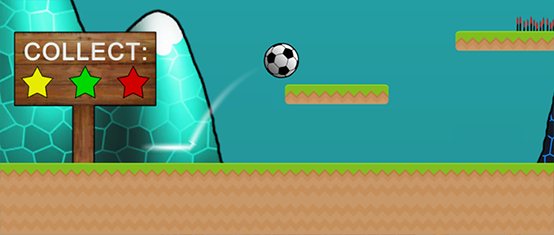
\includegraphics[width=0.3\textwidth]{Pics/gf}
\caption{Players control a rolling ball. Their task is to collect three stars.}
\label{fig:game}
\end{figure}

%Since the aim is to allow for players to experience the game feel as much as possible, the level has been designed to be simple and not too challenging, ensuring that most participants would complete the level without too much trouble.
%To ensure that all participants had comparable experiences, the game was fixed at a 960x600 resolution, no matter if played in a browser or as a standalone program. Also, the camera is set to follow the player avatar directly; however, small deadzones for vertical and horizontal movement were implemented, meaning that the camera will only move when the player moves outside these zones (e.g., by jumping more than a few pixels).